\section{Trend detail}
\label{app:trend}

\subsection*{Signal matrix}

\begin{longtable}[]{@{}lrrrrl@{}}
\toprule\noalign{}
Segment & Slope & Raw $p$ & Holm $p$ & BH $p$ & Reading \\
\midrule\noalign{}
\endhead
Overall & $-0.11$ & 0.921 & 1.000 & 0.989 & no signal \\
CPV-32 & $-0.01$ & 0.989 & 1.000 & 0.989 & no signal \\
CPV-35 & $+0.03$ & 0.923 & 1.000 & 0.989 & no signal \\
CPV-48 & $-0.84$ & \textbf{0.032} & 0.159 & 0.159 & nominal signal only \\
CPV-72 & $+0.70$ & 0.285 & 1.000 & 0.714 & no signal \\
\bottomrule\noalign{}
\end{longtable}

Slopes are ordinary least squares over the last twelve quarters, in awarded episodes per quarter. Five series
are tested simultaneously, so raw $p$-values are reported beside Holm and Benjamini--Hochberg adjustments. The
pre-declared exploratory level is $\alpha = 0.10$ on the raw $p$-value, fixed before the series were fitted
and left unchanged.

\subsection*{PELT change points under three penalties}

\begin{longtable}[]{@{}llll@{}}
\toprule\noalign{}
Segment & Candidate breaks ($\lambda = 0.5$) & $\lambda = 1$ & $\lambda = 2$ \\
\midrule\noalign{}
\endhead
Overall & 2020Q4, 2023Q2 & 2023Q2 & --- \\
CPV-32 & 2020Q2 & 2020Q2 & 2020Q2 \\
CPV-35 & 2019Q1, 2020Q2, 2022Q3 & 2019Q1, 2020Q2 & 2022Q3 \\
CPV-48 & 2024Q1 & 2024Q1 & 2024Q1 \\
CPV-72 & 2021Q1, 2023Q1 & 2021Q1, 2023Q1 & 2021Q1 \\
\bottomrule\noalign{}
\end{longtable}

The penalty is the only tuning knob, and it trades a better fit against more breaks; the practical consequences are reviewed by \citet{truong2020}. A break is called \emph{stable} only when a break lies within one quarter under all three penalties. Three
qualify: CPV-32 at 2020Q2, CPV-48 at 2024Q1, CPV-72 at 2021Q1. The overall series and CPV-35 carry none: their
candidates disappear as soon as the penalty changes. No break is attributed to a cause; PELT dates a level
shift, it does not explain one.

\subsection*{Stationarity}

\begin{longtable}[]{@{}lrrrr@{}}
\toprule\noalign{}
Segment & ADF statistic & ADF $p$ & KPSS statistic & KPSS $p$ \\
\midrule\noalign{}
\endhead
Overall & $-5.890$ & 0.000 & 0.268 & 0.100 \\
CPV-32 & $-6.086$ & 0.000 & 0.808 & 0.010 \\
CPV-35 & $-1.684$ & 0.439 & 0.444 & 0.058 \\
CPV-48 & $-1.749$ & 0.406 & 0.545 & 0.032 \\
CPV-72 & $-5.439$ & 0.000 & 0.611 & 0.022 \\
\bottomrule\noalign{}
\end{longtable}

The two tests carry opposite nulls --- ADF assumes a unit root, KPSS assumes level stationarity --- so they are
read together. Only the overall series gives a clean reading (rejects the unit root, fails to reject
stationarity). The others disagree, which means the series is not cleanly classified over a window this short.
That ambiguity is reported rather than resolved, and nothing in the report depends on resolving it.

\subsection*{Regime model}

\begin{longtable}[]{@{}llrl@{}}
\toprule\noalign{}
Segment & Current regime & Posterior & Mean quarterly change by regime \\
\midrule\noalign{}
\endhead
Overall & growth & 0.750 & decline $-15.5$, plateau $-7.8$, growth $+17.8$ \\
CPV-32 & growth & 0.992 & decline $-12.3$, plateau $-0.5$, growth $+11.6$ \\
CPV-72 & growth & 0.594 & decline $-6.6$, plateau $+0.1$, growth $+7.5$ \\
\bottomrule\noalign{}
\end{longtable}

The three-state Gaussian hidden Markov model is fitted on the quarter-over-quarter \emph{change} in episode
count, not on the level, so its states describe a typical direction of movement rather than a segment's
activity. Because the series are noisy and low-count, the \texttt{plateau} state is a data-driven middle tier
rather than a change centred exactly at zero. A regime label is a model belief about the most recent quarter;
the twelve-quarter slope summarises a different window, and the two need not agree.

\subsection*{Technology series}

\begin{longtable}[]{@{}lrrrrl@{}}
\toprule\noalign{}
Class & Episodes & Slope & Raw $p$ & Holm $p$ & Reading \\
\midrule\noalign{}
\endhead
NETWORK\_TELECOM & 855 & $-0.255$ & 0.515 & 1.000 & no trend detected \\
CYBERSECURITY & 314 & $+0.196$ & 0.463 & 1.000 & no trend detected \\
BUSINESS\_SOFTWARE & 849 & $-0.762$ & 0.248 & 0.992 & no trend detected \\
IT\_INFRASTRUCTURE & 295 & $-0.018$ & 0.901 & 1.000 & no trend detected \\
IT\_SERVICES & 486 & $+0.448$ & 0.194 & 0.972 & no trend detected \\
\bottomrule\noalign{}
\end{longtable}

Technology and CPV series now use the same 43-quarter observation window, 2015Q2--2025Q4; the partial 2015Q1
is excluded from both. As for the CPV analysis, the table reports ordinary least-squares slopes over the most
recent twelve quarters. No technology series shows a recent linear trend before or after correction.

\begin{figure}[htbp]
\centering
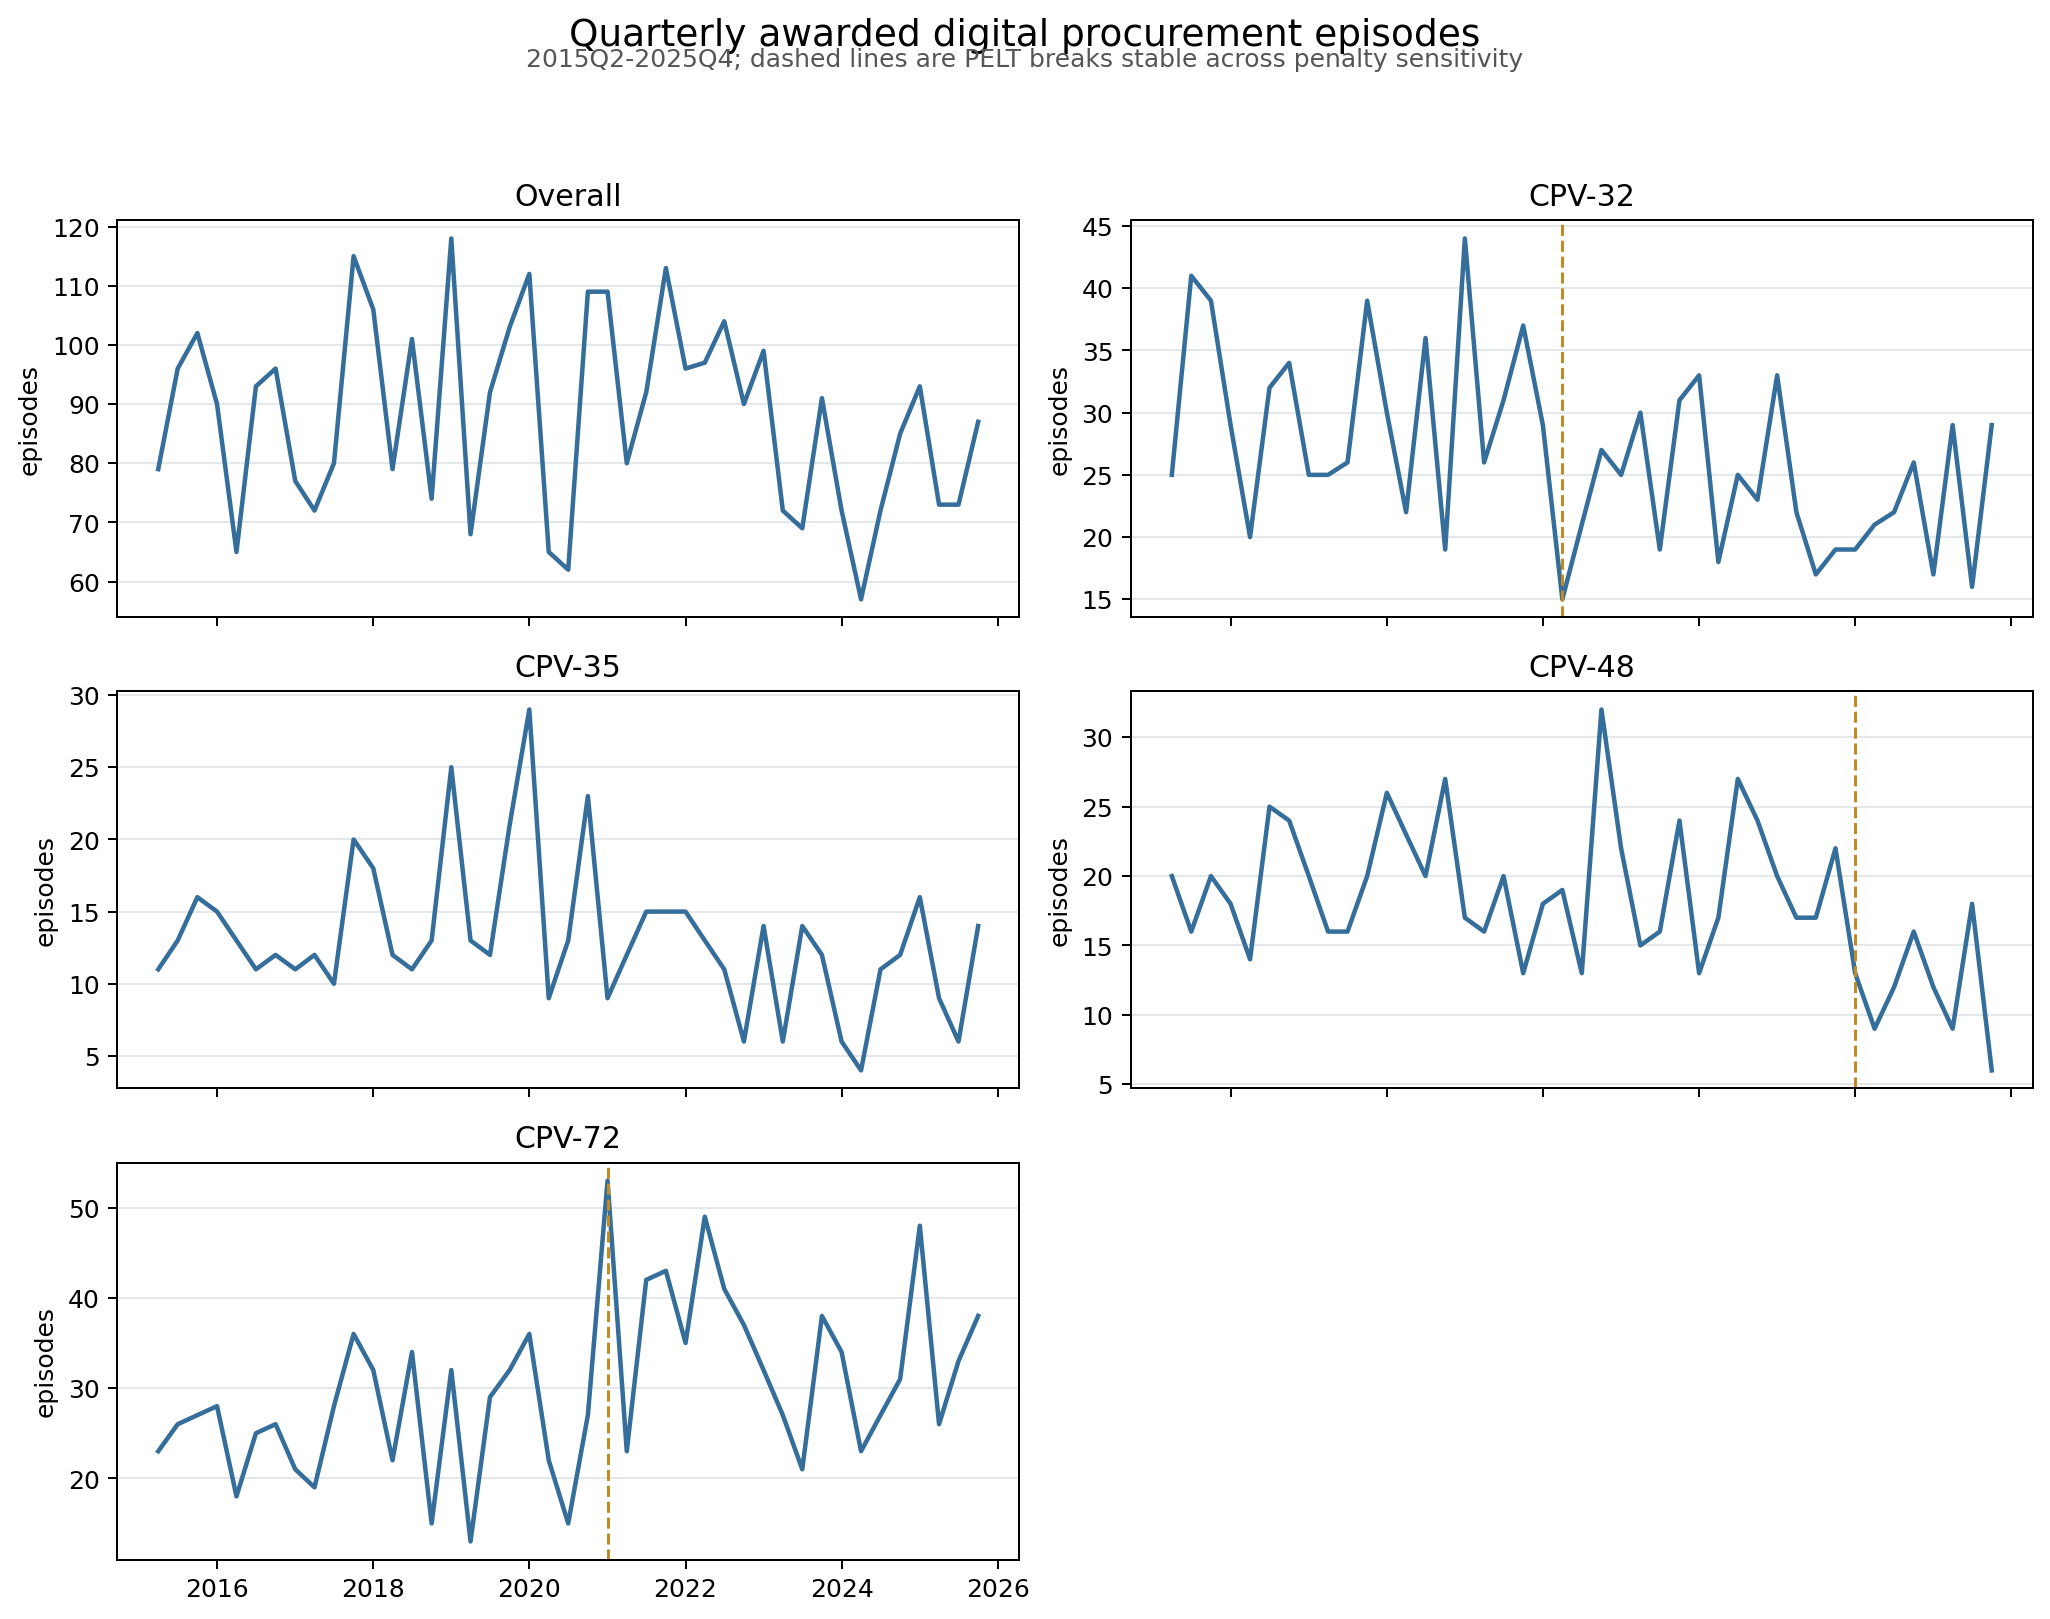
\includegraphics[width=0.95\linewidth]{figures/appF_quarterly_counts.png}
\caption{Quarterly awarded-episode counts, overall and by CPV division. The visual impression of movement in
individual segments is what the slope tests and the multiplicity correction are there to discipline: none of
these series carries a trend that survives correction for the five tests run together.}
\label{fig:appf-quarterly}
\end{figure}

\begin{figure}[htbp]
\centering
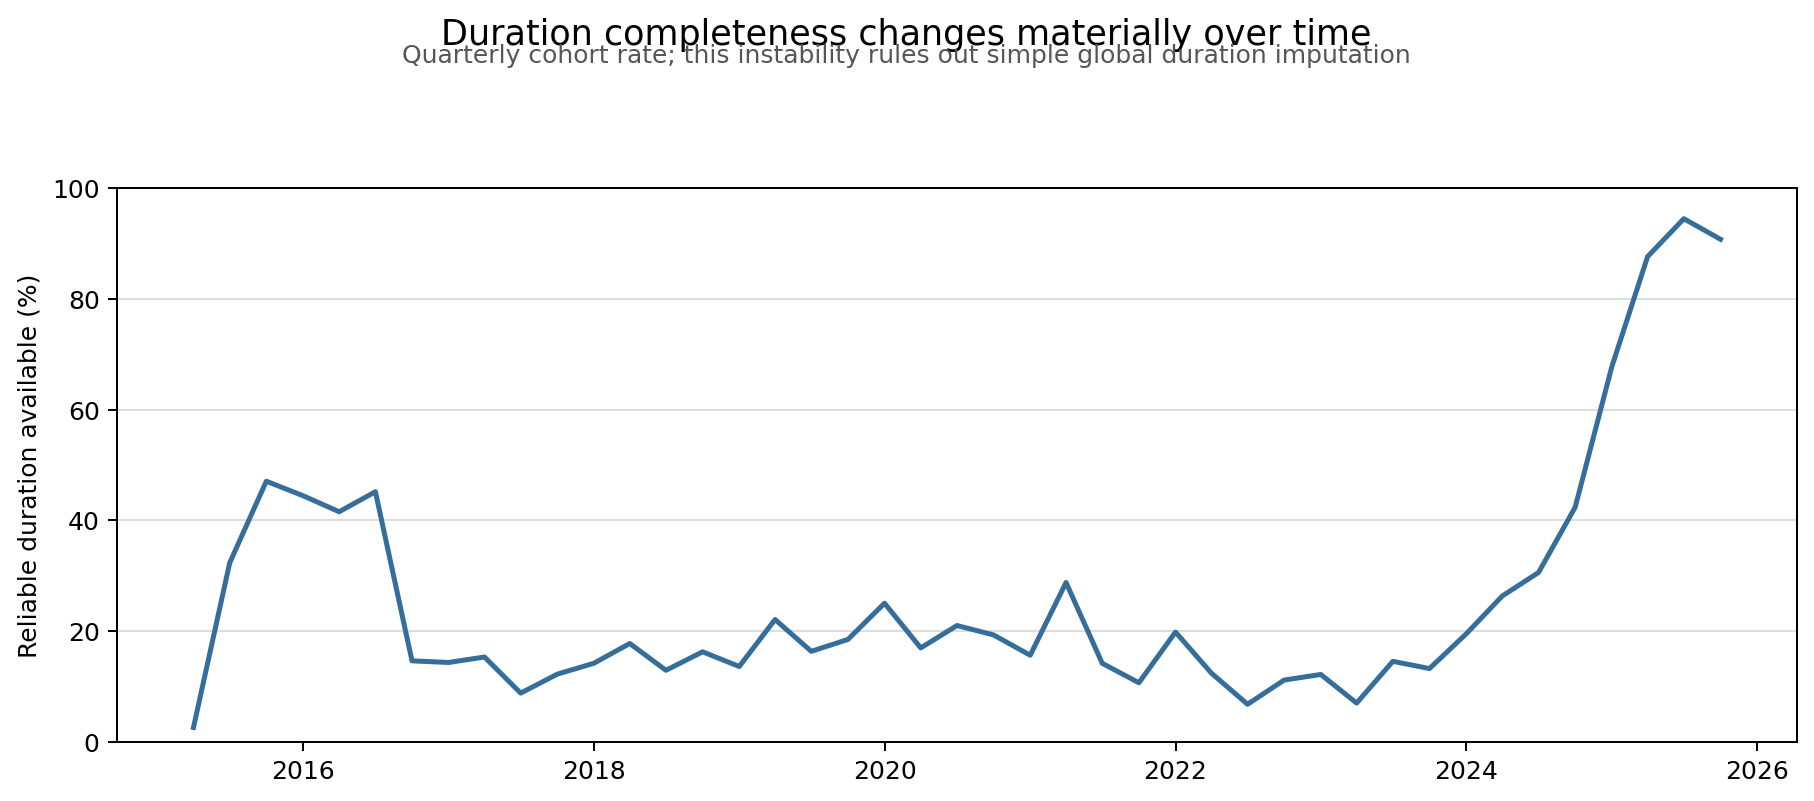
\includegraphics[width=0.78\linewidth]{figures/appF_duration_completeness.png}
\caption{Completeness of the declared-duration field by year. The sharp rise in 2025 is a schema and
completeness change, not evidence that contract durations changed. Median-duration trend claims would mix
periods with substantially different observation processes, which is why no change-point detection is run on
duration values.}
\label{fig:appf-duration}
\end{figure}
